%%%%%%%%%%%%%%%%%%%%%%%%%%%%%%%%%%%%%%%%%%%%%%%%%%%%%%%%%%%%%%%%%%%%
% Grundlagen
%%%%%%%%%%%%%%%%%%%%%%%%%%%%%%%%%%%%%%%%%%%%%%%%%%%%%%%%%%%%%%%%%%%%

\chapter{Background and related work}
  \todo[inline]{Give all the necessary background that is needed to justify and understand the problem and the approach.
  - comment on employed hardware and software
  - describe methods and techniques that build the basis of your work
  - review related work(!)
  - roughly 1/3 of thesis
  }

\section{The Electrical Grid and Flexibility}
% 1. Describe the goals and the structure of the Electrical Grid
The electrical grid is basic infrastructure that enables the function of our modern society.
It connects electricity consumers, from private consumers to heavy industry, with producers.
Historically, the entire system has been built for reliable large-scale power generation, overwhelmingly fuelled by coal and natural gas, together accounting for 67\% of Germany's electricity consumption in 1985, with 27\% provided by nuclear energy \cite{ritchie2022Energy}.

Climate change and the exit from nuclear power require a radical increase in the share of renewable electricity. As of 2021, renewable energy accounts for 40\% of electricity consumption in Germany \cite{ritchie2022Energy}.
An overview of the historical development is shown in figure \ref{fig:electricity_mix}

\begin{figure}
    \centering
    \frame{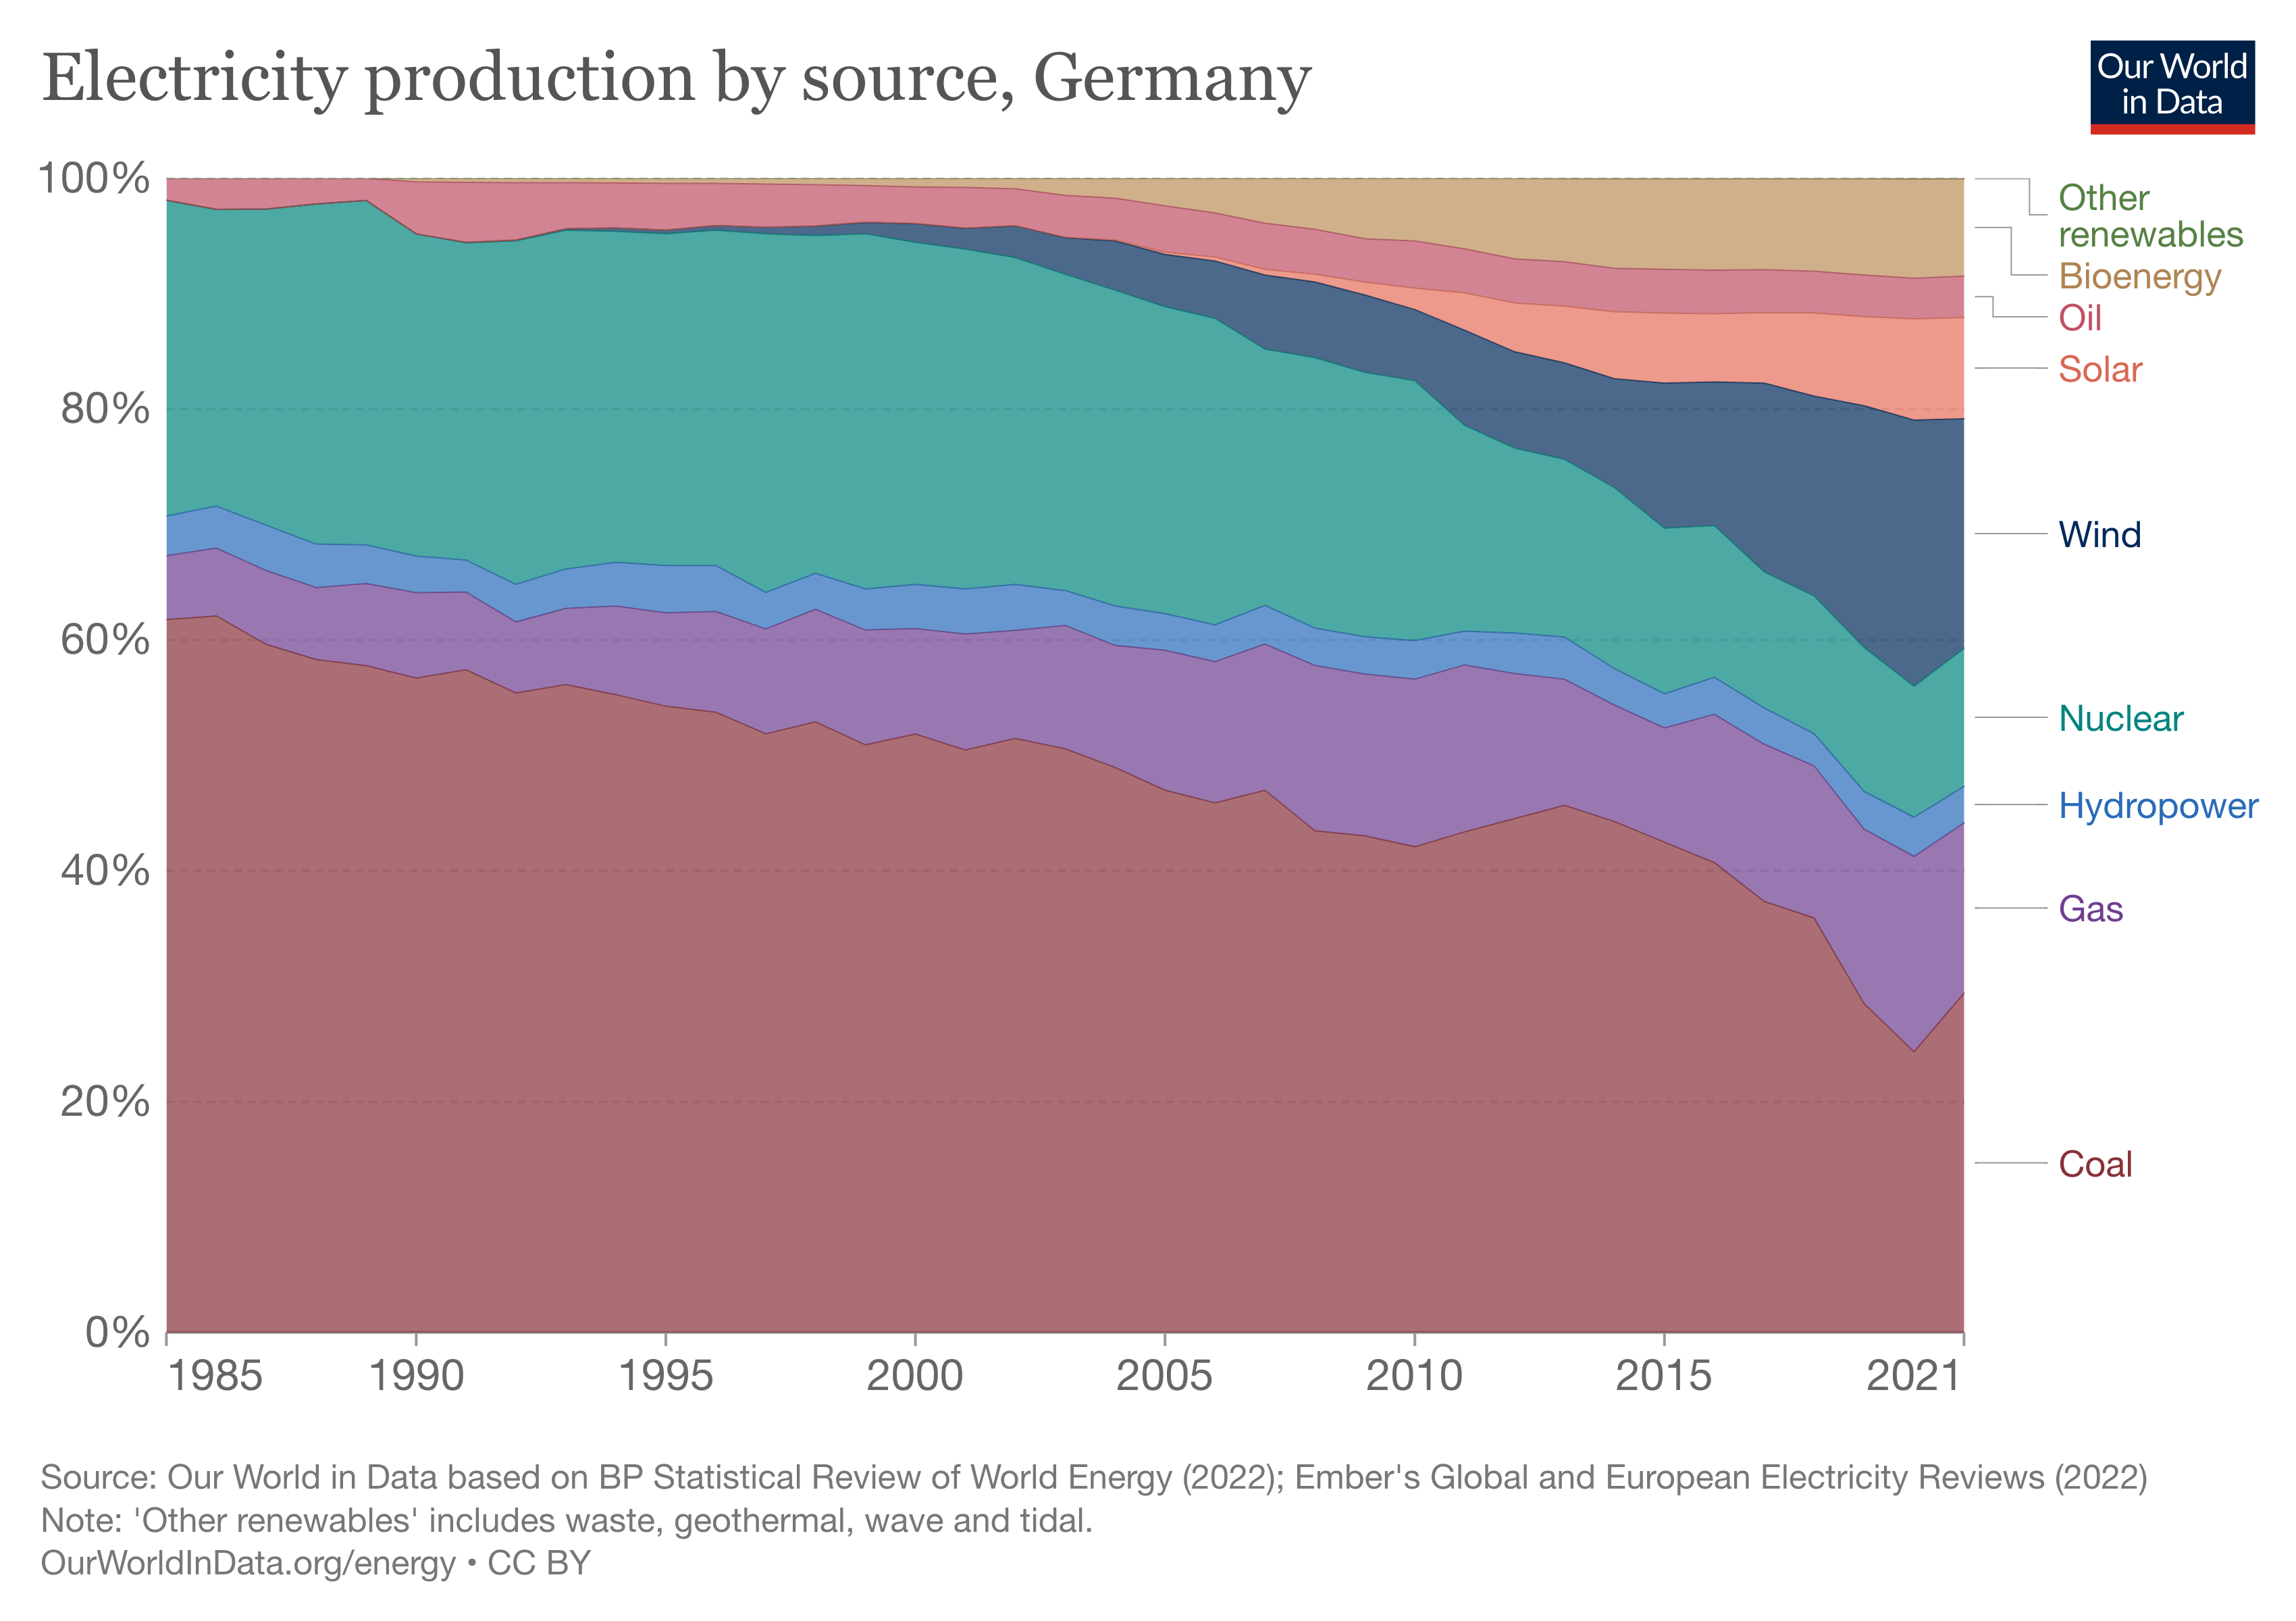
\includegraphics[width=\figurewidth]{figures/electricity_mix.png}}
    \caption{The share of renewable electricity has risen significantly from 1985 to 2021, while nuclear and fossil fuels have declined.}
    \label{fig:electricity_mix}
\end{figure}

While conventional energy generation can flexibly respond to demand, renewable energy depends on the weather.
It is therefore intermittent and harder to predict, see figure \ref{fig:flexibility}. To be able to meet demand, there is a new need for flexible backup power.
Natural gas plants are more environmentally friendly than coal plants and can be flexibly turned on and off in a matter of minutes.
As a result, the share of electricity powered by natural gas has risen along with renewables.

\begin{figure}
    \centering
    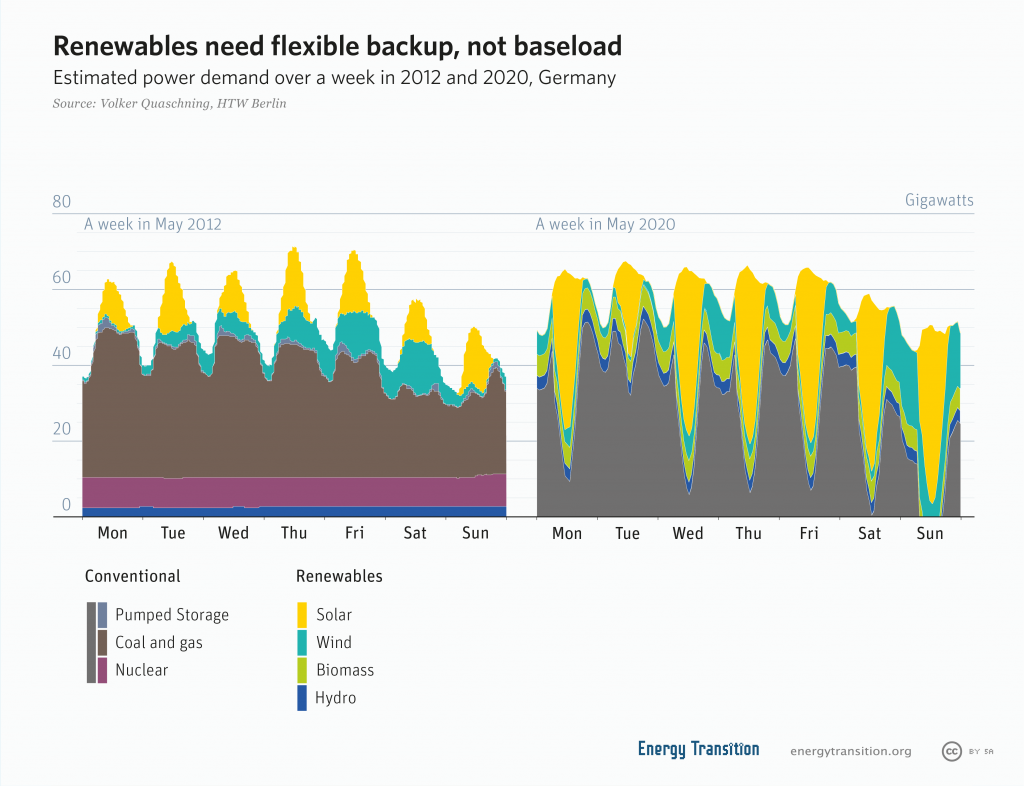
\includegraphics[width = \figurewidth]{figures/flexible_renewables.png}
    \caption{Renewable electricity is intermittent and hard to predict precisely. As the share of renewable electricity increases, the electrical grid needs to respond flexibly to meet demand.}
    \label{fig:flexibility}
\end{figure}


% 2. Describe Challenges posed by the energy transition
Another aspect of the energy transition is the electrification of many processes which previously used fossil fuels directly.
Internal combustion engine cars are being replaced by more efficient battery-powered electric cars and heating units that use natural gas or oil are being replaced by much more efficient electric heat pumps.
Many heat pumps can also be run in reverse to cool a building, which climate change makes more and more necessary, but this enables additional electricity demand in the summer.

The ongoing energy transition puts a lot of pressure on the grid.
On the one hand, the electricity supply is becoming less reactive, while on the other hand, many polluting processes are being electrified, causing additional demand.\todo{maybe give specific number}
During large future demand spikes, the total load on the grid could exceed current capacity. To cope, new transmission lines are being built, a costly and complicated process.

In order to both reduce reliance on fossil fuels and to keep the total load below grid capacity, there is a need for additional flexibility in the system.
A traditional source of flexibility has been pumped hydropower storage.
When there's unused electricity, it can be stored by pumping water uphill.
When needed, water can be released and used to generate electricity. 
Hydropower depends almost entirely on geography. There is almost no potential to develop more hydropower storage.

A different large-scale method of energy storage is batteries, which have only found limited use due to their cost. Hydrogen can also be used as a way to store and even transport energy, with several chemical processes currently being explored.
However, this method is also costly, and any produced hydrogen is probably worth more as a crucial chemical than as pure electricity storage.\todo{rephrase, cite}

As flexibility in electricity supply decreases, and centralized storage facilities remain too expensive, electricity demand needs to become more flexible.


\section{Demand Response}
% 3. Demand Side Flexibility
Both the inflexibility of renewable power generation and the limited capacity for centralized flexible energy storage leave one component of the electric system: In a renewable-dominated grid, demand needs to flexibly respond to changes in available supply.
In order to stabilize the grid, grid operators employ schemes to curb demand in case of exceptionally large pressure on the grid.
Large industrial consumers are paid in advance for shutting off their processes if needed.
As a matter of last resort, rolling blackouts are introduced to curb demand when electricity production can not keep up with consumption.
An electric grid designed for renewable energy needs more fine-grained coordination across a larger fraction of demand.

In order to implement demand response, electricity consumers need to be incentivized and able to adapt their processes to available supply.
Proposed incentive schemes for demand response include market-based solutions that feature a flexible electricity price and solutions of centralized control that pay out flat rewards for participation, as well as combinations of the two. \todo{cite}
In order to be able to react to changes in demand, electricity-consuming processes need to be aware of the current and future available supply.
This can be a human in the loop, deciding to shift a process to a time with cheaper electricity, or this can be automated.
For example, a private prosumer that produces solar electricity might prefer to run their washing machine only on sunny days when electricity is free to them.
However, this means the human needs to keep track of the weather and is put under additional cognitive load when planning this.

As stated before, the process of heating is being electrified.
While this increases the load on the electric grid, it is also a chance to provide flexibility:
When equipped with an intelligent and connected control system, the heating system can flexibly react to changes in price, using hot water tanks or the building itself as heat storage.
Similarly, when intelligently automated, the charging process of an electric car or a home battery can somewhat react to market conditions.
\todo{somehow mention coordination goals}

Technologically, this amounts to a control problem:
The controller's goals are to meet certain demands (like ensuring a comfortable living temperature) while minimizing cost. In the context of the larger system, there is the shared goal of coordination between different electricity-consuming processes.
This involves both an understanding of the dynamics of the controlled system and an understanding of how prices are likely to change.
Different technological approaches can be employed for this.
When system dynamics are known and prices change predictably, for example with fixed rates per time of day, an optimal rule-based controller can be derived. \todo{cite and make sure this is true!}
A rule-based controller has the advantage of being transparent and reliable, but it's not flexible enough to react to changing system and pricing dynamics.
Several adaptive control algorithms have been proposed for use in demand response. \todo{List some and cite}
\missingfigure{illustrate control problem}
\todo[inline]{
    notes on this section:
        - focus more on buildings
        - use the following review paper:
        - \cite{li2021EnergyFlexibilityResidential}, a review paper about energy flexibility in residential buildings
}


\section{Reinforcement Learning}

\todo[inline]{
    1. Explain RL Fundamentals
        1. Markov Decision Process
            1. Highlight stochasticity of transition and Reward functions
            2. Reward function?
            3. Mention generalizations: POMDP, (Multi-Agent MDP?), Non-stationary MDP
        2. Value Learning
            - Introduce the notion of a state value
            - Bellman updates
            - Q-Learning
            - Mention Policy Gradient methods
        3. Deep Q-Learning
            - introduce Fundamentals of Deep Learning? Deep RL is somewhat like using a POMDP?
            - Introduce further tricks employed by DQN
                - Replay Buffer
                - Dueling Q-Networks?
                - TD-Learning / Target Network
        4. Importance of Action Selection and Exploration strategies
            - Exploration vs. Exploitation Dilemma
            - Convergence guarantees
}


% 1. RL Fundamentals
\subsection{Reinforcement Learning Fundamentals}
Reinforcement Learning (RL) is a feedback-based learning paradigm derived from behavior learning in animals.
This section serves as a brief introduction to the topic.
Unless otherwise stated, this section is based on the textbook \cite{sutton2018ReinforcementLearningIntroduction}.
In Reinforcement Learning, there is a clear distinction between the learning agent and the environment.
The agent is able to observe the state of the environment and perform an action.
In turn, the environment is affected by the action and transitions into a new state according to its stochastic transition dynamics.
The environment passes the resulting state and a reward signal back to the agent.
Typically, the agent's goal is to select actions that obtain the maximum reward.
In an infinite environment, the objective is to maximize the expected value of the total discounted future reward.

The environment specifies the entire reinforcement learning task.
Formally, it is a discounted Markov Decision Process (MDP):
$$ \text{MDP} = (S, A, R, \gamma, p),$$
where $S$ is the set of possible states, $A$ is the set of possible actions, $R$ is the set of possible rewards, $\gamma$ is the discount rate and $p(s', r|s,a)$ is the probability distribution that specifies the environment dynamics.
It is important to note that an MDP has the Markov Property, i.e. the dynamics depend entirely on the state and action, there is no hidden state.
The state space can therefore also be called the observation space.

When modeling a real-world control problem, an MDP necessarily is a simplifying assumption.
In reality, state transitions often depend on outside influences or are non-stationary for other reasons.
In complex problems, the desired behavior is not obvious. Therefore, designing the reward function is often non-trivial.

\todo{Mention a few RL applications that can be used as examples}
\todo{Mention exploration/exploitation-dilemma here}

% 2. Towards DQN
\subsection{Q-Learning}
% - Value Learning
Some environment states are preferable to others.
Value Learning is a class of RL algorithms that builds on this intuition.
From a trajectory of state-action-observation-reward tuples that were generated while following a policy $\pi$, a Value Learning algorithm assigns each state the expected future discounted reward that will be received when the agent, in state $s$, continues to act according to $\pi$:

$$v_\pi(s) = \mathbb{E}[G_t | S_t=s] = \mathbb{E}[\sum_{k=0}^{\infty}\gamma^kR_{t+k+1} | S_t = s], \text{for all } s \in S$$

Similarly, one can define the value of taking an action in a certain state:
$$ q_\pi(s,a) = \mathbb{E}[G_t | S_t=s, A_t = a] = \mathbb{E}[\sum_{k=0}^{\infty}\gamma^kR_{t+k+1} | S_t = s, A_t = a]$$

This Action-Value Function or Q-function induces a greedy policy by evaluating $q(s,a)$ for the current state and all possible actions, and selecting the highest-expected reward action.
For the optimal policy $\pi_*$, the greedy policy induced by $q_{\pi_*}$ is $\pi_*$ itself.
For more detail on how the optimal policy can be approximated, please refer to \cite{sutton2018ReinforcementLearningIntroduction}.

%explain (e-greedy) action selection
%explain Q-Learning
A process that iteratively improves an initial Q-function is Q-Learning.
Its basic idea is that the Q-function can induce a better greedy policy than the one with which it was generated.
A Q-Learning step consists of taking an action $a$ in state $s$ according to the current greedy policy and performing a Bellman update on $q(s,a)$, using $\max_a{q(s',a)}$.
However, a slight modification needs to be made: To make sure all possible trajectories are explored, the $\epsilon$-greedy policy is used instead, which acts randomly with a small probability of $\epsilon$, and acts greedily otherwise.

\todo[inline]{
    Focus less on the idea of value learning.
    Instead, explain Tabular Q-Learning better
}

% - Deep Q-Learning
\subsection{Deep Q-Network}
\cite{mnih2015HumanlevelControlDeep} propose the Deep Q-Network algorithm (DQN), which is able to learn and play many video games better than humans.
DQN is a Q-Learning algorithm that acts according to an $\epsilon$-greedy policy.
It approximates the Q-function using a deep convolutional neural network, which is able to store complex information like video game dynamics.
The deep Q-network is optimized during every optimization step using stochastic gradient descent.

In order to arrive at a stable and efficient algorithm, DQN makes use of two notable modifications to standard online Q-Learning:
The first one, Experience Replay, stores past trajectories in a replay buffer.
During every optimization step, a minibatch of transitions $(s, a, r, s')$ is sampled from the replay buffer and used to compute the loss and gradient for the optimizer step.

The second modification is the use of a separate target Q-network.
The loss that is minimized is
$$ ((R_j + \gamma \max_a{\hat{q}(s',a)}) - q(s,a))^2$$
Instead of using the Q-network $q(s',a)$ as the target Q-value, DQN uses $\hat{q}(s',a)$.
$hat{q}$ is a lagging copy of the Q-network that is updated after several optimization steps.
This improves the stability of the algorithm.



% Uncertainty, Exploration vs Exploitation
\subsection{The Reward Distribution}
\todo[inline]{
    - Introduce the idea of Thompson sampling
        - requires a distribution instead of an expected Q-Value.
            - give formula for the q-distribution
    - Learn distributions: QR-DQN and \cite{azizzadenesheli2018EfficientExplorationBayesian}
    - 
    - If you do not have uncertainty, what can you do?
    - decay epsilon
    - use boltzmann sampling
    - Talk about how DQN treats uncertainty. (With epsilon-decay)

    - Introduce epistemic and aleatoric Uncertainty and their significance for action selection.
        - The uncertainty in the learned return distribution is caused both by inherent stochasticity of the environment and epistemic uncertainty.
        - Optimal action selection depends only on the epistemic uncertainty. If the goal remains to maximize the expected return overall, risk-averse things should happen too.
        - mathematically define them (variance of the Q estimator?)
        - \cite{hullermeier2021AleatoricEpistemicUncertainty} explain the concept.
        - 

}

Reinforcement Learning algorithms need to solve the Exploration/Exploitation-Dilemma.
When interacting with the environment, they need to balance between the value of gathering new information and the value of acting greedily according to their current knowledge.
The $\epsilon$-greedy policy exposes the parameter $\epsilon$ as a direct way to control this trade off.
Because the algorithm has the most to learn at the beginning, $\epsilon$ is commonly set to a high value in the beginning and then decayed over time.
Most Reinforcement Learning algorithms don't provide an explicit measure of uncertainty, which could be used to dynamically adapt this practice to the environment at hand.


\section{Reinforcement Learning for Building Demand Response}
\todo[inline]{
- Motivation: RL is a class of control algorithms that has been successfully applied to DR.
- Why is building DR a particularly good fit for RL?
- Mention prior work: When has RL been applied to building demand response?
    - paper 1: 
    - paper 2: 
    - paper 3: 

    - (Mention related work: applied algorithms and their results)
    - (Other Frameworks and available data, including CityLearn, real-life applications)
}

\subsection{CityLearn} % The basis for the environment.
\todo[inline]{
    1. Introduce and Explain CityLearn (cite)
        - What is it?
            - A simulation framework for constructing demand response environments for RL
        - What are its main contributions?
            - Provide an accessible entry point for RL researchers for DR (cite 2021 challenge paper)
            - Validate the usefulness for RL methods
            - Can use Real-World Data
            - Limited application as Benchmark suite
    2. CityLearn has previously been approached in a number of ways.
        - paper 1
        - paper 2
        - paper 3
}
One particularly interesting framework for RL in demand response is CityLearn.



















% \todo[inline]{
%     2. Related Work
%         1. Uncertainty-Aware Reinforcement Learning: Related Work
%             - Uncertainty-Aware Machine Learning Methods: Distributions instead of estimators
%                 - Explicitly model input uncertainty.
%                     - Assume a distribution, model parameters
%                     - e.g. Discrete distribution, normal distribution, beta distribution, or general distribution parameterized by quantiles.
%                     - Example in RL: POMDP
%                     - Algorithms: Bayesian NN, Gaussian Processes, Variational Autoencoders (uncertainty about deep representation)
%                     - Advantages: More robust
%                     - Disadvantages: More expensive, need to model data generation process
%                 - Explicitly model output uncertainty.
%                     - In classification: Confidence score (discrete distribution), class probabilities
%                     - In regression: Again, model distribution and parameters
%                     - Examples: Bayesian NN, Ensemble models, Distribution Learning, *UA-DQN*
%                     - Advantages: More trustworthy and more useful for risk-aware decision-making, more robust, can be more sample-efficient
%                     - Disadvantages: more expensive, more complex, less robust
%             - Examples of Uncertainty-aware RL applications:
%                 - TODO
% }





% \clearpage
% ------- Erster Entwurf below ------


% \section{Uncertainty in Reinforcement Learning}
% \todo[inline]{Introduce Uncertainty terms and formalisms from different perspectives. Then apply to RL.}
% There is a rich body of work on uncertainty. Mathematical and statistical notions of uncertainty, perspectives from economics for decision making under uncertainty.

% Notes:

% - Motivation: Most information is uncertain to some extent. Making good decisions under uncertainty requires an awareness of the uncertainty.
% - Uncertainty vs Risk: Uncertainty is a measure of the information content of a random variable or an observation???, Risk is the cost associated with different situations.
% - formal framework (maybe borrow from Econ: When to buy or sell a given asset?)
% - Decision making under uncertainty
%     - which objective (Expected value vs risk metrics)
% - different types of uncertainty (e.g. aleatoric vs epistemic)
%     - there are different types of uncertainty: Some uncertainty can be reduced by learning more about the problem, other uncertainty can not.
%     - this stems from the formulation of RL as a stochastic MDP
%     - for example, a biased coin. You will be able to learn something about it, but not actually predict the outcome ???

% Uncertainty in RL: (maybe this should already be in approach?)
% - How is Uncertainty commonly modelled?
%     - epistemic uncertainty in the observations: not explicitly modelled, somewhat represented in state-value function
%     - stochasticity in the environment dynamics (+consequences of actions): accepted in the MDP. learned as transition probabilities in model-based RL, subsumed in e.g. Q-function in model-free RL.
%     - epistemic uncertainty in the environment dynamics: modelled as transition probabilities
%     - stochasticity in the reward function: not usually explicitly modelled
%     - epistemic uncertainty in the reward function: modelled implicitly in the state-value function
%     - uncertainty about causality? - probably not really relevant? should I discuss it somewhere else?
% - Adaptations for explicit treatment of uncertainty:
%     - Formalism for non-perfect observations: POMDP (usually there are hidden variables) -> Usually solved by estimating an MDP, solving that.
%         - POMDP does not assume the Markov property on observations, but does assume a hidden MDP
%     - ???
%     - RL from human preferences? (for learning a reward function)
% - Benefits of explicit treatment of uncertainty/Motivation:
%     - Risk-aware strategies
%     - better performance (maybe? TODO: Test this)
%     - more robustness (possibly? TODO: support this or not)
%     - better interpretability (possibly?)
%     - TODO: other
% - Drawbacks:
%     - more complex models require more training data
%     - less efficient algorithms
%     - not as well understood theoretically
%     - might perform worse than just learning everything implicitly!
    
% Risk-aware strategies:
%     - can either specify a risk tolerance at time of inference or during training
%     - during training: change reward function
%     - at time of inference: requires model of the environment (I think) or a Q-function
%     - more robust: can hand over control to e.g. humans when uncertain
    
% Uncertainty in Multi-Agent Learning: (maybe exclude this completely)
%     - Multi-Agent Environments are characterized by simultaneous actions by multiple agents, who each learn and act according to their own rewards.
%     - More realistic and resilient than centralized control
%     - absent trust, might be stuck in a suboptimal equilibrium



  